\documentclass[a4paper]{article}

%% Language and font encodings
\usepackage[english]{babel}
\usepackage[utf8x]{inputenc}
\usepackage[T1]{fontenc}

%% Sets page size and margins
\usepackage[a4paper,top=3cm,bottom=2cm,left=3cm,right=3cm,marginparwidth=1.75cm]{geometry}

%% Useful packages
\usepackage{amsmath}
\usepackage[table,xcdraw]{xcolor}
\usepackage{graphicx}
\usepackage[colorinlistoftodos]{todonotes}
\usepackage[colorlinks=true, allcolors=blue]{hyperref}
\usepackage{amsmath}
\usepackage{tikz}
\usepackage{tkz-tab}
\usepackage{caption}
\usepackage{latexsym}
\usepackage{amssymb}
\usepackage{amsmath}
\usepackage{subcaption}
\usepackage{mathtools}
\usepackage{multirow}
\usepackage{listings}
\usepackage{color}

\definecolor{mygreen}{rgb}{0,0.6,0}
\definecolor{mygray}{rgb}{0.5,0.5,0.5}
\definecolor{mymauve}{rgb}{0.58,0,0.82}

\lstdefinestyle{customc}{
  belowcaptionskip=1\baselineskip,
  breaklines=true,
  frame=L,
  xleftmargin=\parindent,
  language=C,
  showstringspaces=false,
  basicstyle=\footnotesize\ttfamily,
  keywordstyle=\bfseries\color{green!40!black},
  commentstyle=\itshape\color{purple!40!black},
  identifierstyle=\color{blue},
  stringstyle=\color{orange},
}

\lstdefinestyle{customasm}{
  belowcaptionskip=1\baselineskip,
  frame=L,
  xleftmargin=\parindent,
  language=[x86masm]Assembler,
  basicstyle=\footnotesize\ttfamily,
  commentstyle=\itshape\color{purple!40!black},
}

\lstset{escapechar=@,style=customc}

\usetikzlibrary{automata,arrows,positioning,calc}
\usetikzlibrary{shapes,snakes}
\DeclarePairedDelimiter\abs{\lvert}{\rvert}

\title{[TUTORIAL] KOMONDOR: A Wireless Network Simulator Based on COST}
\author{Sergio Barrachina and Francesc Wilhelmi}

\begin{document}
\maketitle

\begin{abstract}
Komondor is a wireless network simulator that will allow Barrachina and Wilhelmi to understand the behavior of wireless network contention operating in different power (TPC and CCA) and different channels (DSA and DCB). 
\end{abstract}

\tableofcontents

%-------------------------------
%-------------------------------
%-------------------------------
%-------------------------------

\section{Introduction}
Komondor is an event-based simulator based in COST \cite{ref:cost}, a simulator SENSE\footnote{SENSE main website: \url{http://www.ita.cs.rpi.edu/}}...
% * <francisco.wilhelmi@upf.edu> 2017-05-31T15:53:22.000Z:
% 
% TODO: Talk about new requirements in WLANs and proposed solutions (emphasize IEEE 802.11ax standard).
% 
% ^.

% * <francisco.wilhelmi@upf.edu> 2017-05-31T15:53:17.111Z:
% 
% TODO: Talk about the application of AI to WLANs to enhance their performance
% 
% ^.

% * <francisco.wilhelmi@upf.edu> 2017-05-31T15:53:10.432Z:
% 
% TODO: Argue about the need of building Komondor based on lack of simulation tools and adaptability of learning mechanisms to them.
% 
% ^.
We have decided to build a new simulator for the impediments shown by ns-3, at which it is not possible to simulate the new IEEE 802.11ax functionalities. In addition, Komondor is intended to support the inclusion of agents for deciding the behaviour of WLANs by using Reinforcement Learning (RL).

Its main features are:
\begin{itemize}
\item CCA
\item Channel Bonding
\item Collisions\^{*}
\end{itemize}

% * <francisco.wilhelmi@upf.edu> 2017-05-31T15:53:40.608Z:
% 
% TODO: Paper structure
% 
% ^.

%%%%%%%%%%%%%%%
% SYSTEM MODEL
%%%%%%%%%%%%%%%
\section{System Model}
\label{section:system_model}
In this Section we describe the models defined for simulating the different layers of the communication between devices.

\subsection{Traffic Modelling}
\label{section:traffic_modelling}
In order to represent an acceptable Downlink traffic model, we have considered that only the APs are able to transmit data packets to the STAs. Regarding traffic generation, we have considered three different models:
% * <francisco.wilhelmi@upf.edu> 2017-05-18T16:36:46.461Z:
% 
% This is a test
% 
% ^ <francisco.wilhelmi@upf.edu> 2017-05-31T15:34:02.511Z.
\begin{itemize}
\item Full buffer: the transmitters are in a permanent saturation regime, so that there are always packets to be sent.
\item Poisson: packets are generated according to a Poisson distribution, at which the time between packets $\Delta_p$ is determined by the packets generation rate $\lambda$, and is given by Equation \ref{eq:poisson_packet_generation}.
\begin{equation}
\label{eq:poisson_packet_generation}
	\Delta_{\rm p} = e^{1/\lambda}
\end{equation}
\item Deterministic: with this model packets are generated at fixed time intervals $\Delta_d$ given by the packets generation rate (shown in Equation \ref{eq:deterministic_packet_generation}).
\begin{equation}
\label{eq:deterministic_packet_generation}
	\Delta_{\rm d} = 1/\lambda
\end{equation}
\end{itemize}

\subsection{Medium Access Control}
\label{section:medium_access_control}
When an AP has a packet to be sent, it implements Carrier Sense Multiple Access with Collision Avoidance (CSMA/CA) to access the medium, in which transmissions are carried out if the channel has been empty for a given BackOff (BO) time. We consider that the channel is empty if the interference in it is equal or higher than a Capture Effect threshold, which allows defining the frequency at which packet losses occur, regardless on the Modulation Coding Scheme used. In Figure \ref{} it is shown an example of CSMA/CA implementation for two WLANs that sense each other, i.e., if one transmits, the other senses the channel as busy.

TO DETAIL A FLOW CHART!!!!!!!!!!!!!!!!!!!\\

As it is shown, AP 1 transmits first since its BO time was lower than for AP 2. After the packet transmission is done, the STA 1 waits for a Short InterFrame Space (SIFS) before sending the ACK, so the AP 1 knows that either the packet or the ACK have been lost after the SIFS time has been exhausted. Once the transmission from AP 1 to STA 1 has finished, and before the AP 2 BO is resumed, it is required to wait for a DCF InterFrame Space (DIFS) time period, which avoids decreasing the BO between a packet and an ACK transmission. At the moment AP 2 starts decreasing the already frozen BO, the AP 1 generates a new BO for doing the next packet transmission.

\subsubsection{Binary Exponential Backoff (BEB)}
\label{section:beb}
The process of generating a BO when a packet transmission is pending is determined by the Congestion Window (CW) and the generation PDF used, which has been considered to support both deterministic and exponential distributions.

Regarding the implementation it has been considered to provide two different ways of generating the BO. The first one assumes that the BO is continuous, so that the probability of noticing a collision by BO is practically null, while the other assumes a discrete BO, so that devices are synchronized and collisions by BO are feasible to occur (depend on the congestion window and the number of coexisting nodes).

\begin{itemize}
\item Continuous Backoff: TODO: Explain how continuous backoff is implemented
\item Discrete Backoff: TODO: Explain how discrete backoff is implemented
\end{itemize}

\subsection{Channel Modelling}
TODO: Explain path-loss models and co-channel interference model

\textbf{Co-channel interference}: it is considered to occur by decreasing 20 dBr by each channel distance (relative dB (dBr) -> if using dBm, it would be -20 dBm).

\textbf{Received power}: Incoming power is assumed to be the same during the entire transmission. This relaxation allows us determining easily whenever the channel of interest is busy or not. A direct implication of it affects to Path-loss models used, as well as some of them assume random variations of the medium, preventing to obtain the same result at different power received calculations (so far, power received is added and subtracted when the node accesses and leaves the channel, respectively). Thus, for each node we store its incoming power (which is computed only once) for subtracting it at the end of its transmission. 



\section{Collisions Modelling}
TODO: Explain how collisions are computed and the Hidden nodes detection

\textbf{Collisions}: collisions in Komondor may be caused by two events:
	\begin{itemize}
	\item \textbf{Deterministic backoff}: these collisions occur when two or more nodes start transmitting at the same time in a shared channel. They cannot occur if the backoff is generated through an exponentially distributed random variable. \textcolor{red}{To be discerned what to do in the deterministic (and real) case.}
    \item \textbf{Hidden and exposed node}: as shown in Figure \ref{fig:collisions_hidden_node}, two or more nodes which are not in coverage of each other, may transmit to the same node sharing part of the channel, which causes a collision. Such collision can be detected by the destination node and act accordingly (NACK to be developed).
    	\begin{itemize}
    	\item How to determine if a transmission can be decoded? Just $P_{rx}>\text{CCA}$? \textbf{NO!}. With SNR! --> get error probability
        \item If the sum of powers (except power of interest) in the channels used in the TX is less than CCA, there is no collision. $P_\text{channel} - P_{rx} < \text{CCA}$
    	\end{itemize}
    
    \begin{figure}
      \centering
      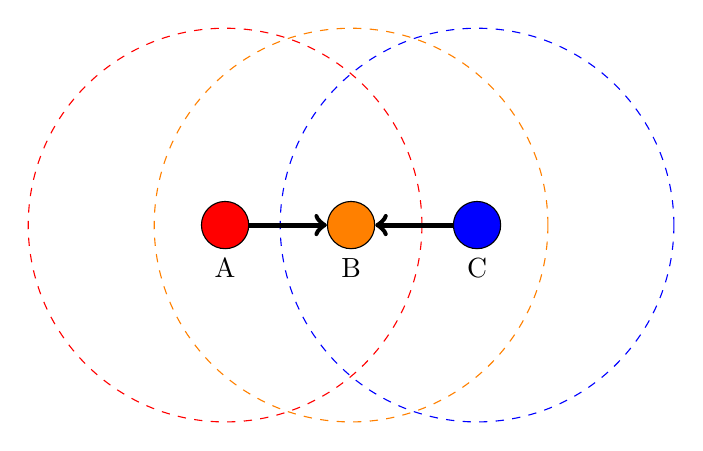
\begin{tikzpicture}
      \node at (0,0) [circle, fill=red, draw, minimum width=0.6cm,minimum height=0.6cm, label=below:$\text{A}$] (A) {};
      \node at (A) [circle,draw=red, minimum size=5cm, dashed] (Ac) {};
      \node[circle, fill=orange, draw, minimum width=0.6cm,minimum height=0.6cm, label=below:$\text{B}$] (B) [right of=A, xshift=0.6cm] {};
      \node at (B) [circle,draw=orange, minimum size=5cm, dashed] (Bc) {};
      \node[circle,draw, fill=blue, minimum width=0.6cm,minimum height=0.6cm, label=below:$\text{C}$] (C) [right of=B, xshift=0.6cm] {};
      \node at (C) [circle,draw=blue, minimum size=5cm, dashed] (Cc) {};
      
      \draw [->,line width=1.8pt] (A) edge (B) (C) edge (B);

      \end{tikzpicture}
      \caption{Hidden \& exposed node cause of collision.} \label{fig:collisions_hidden_node}
      \end{figure}
	\end{itemize}

\begin{figure}
	\centering
  \includegraphics[scale=0.7]{img/ACK_issue.png}
  \caption{Weird case when collisions occur due to last transmitting AP checks the channel right in the SIFS period of other WLAN and picks a range affecting the previous transmission.}
  \label{fig:boat1}
\end{figure}

%%%%%%%%%%%%%%%
% MAIN FEATURES
%%%%%%%%%%%%%%%
\section{Main Features}

\subsection{Modulation Coding Schemes}
TODO: Explain how MCS is done and automatically adjusted (is it?)

\textbf{Modulation Code Scheme (MCS):} We have used the MCS used in IEEE 802.11ax (more info here: \url{https://en.wikipedia.org/wiki/IEEE_802.11ax}). The TX time is going to be determined by the data rate provided by the MCS and the size of the packet to be transmitted. IMPORTANT: by now, it is assumed that all nodes transmit data packets of size 12.000 bits and ACKs of size 112 bits.

The MCS is negotiated before the first transmission of a packet for each of the possible destinations, so that a \textbf{virtual event} is generated in order to devise at the receiver which modulation can be used for each number of channels used according to the power received (which depends on the distance and the path-loss effect).

\textbf{Receiver Driver Protocol:} It is assumed that the Transmitter (TX) knows the Modulation Coding Scheme (MCS) to be used during a transmission with the Receiver (RX). This simulates the Receiver Driver Protocol, at which few symbols are transmitted at the lowest bit-rate for all the subcarriers. Thus, according to the SIRN perceived at the RX, the MCS is chosen and communicated to the TX. The thresholds for each MCS are described in Table \ref{tbl:sinr_thresholds_mcs}

\begin{lstlisting}
/* Add power received when Node X starts transmitting */

for(int c = notification.left_channel; c <= notification.right_channel; c++) {
	channel_occupancy[c]=1;		
	power_received_per_node[notification.source_id] = pw_received_mw;
	channel_power[c] += pw_received_mw;
}

...

/* Subtract power received when Node X stops transmitting */

for(int c=notification.left_channel; c <= notification.right_channel; c++) {
	channel_occupancy[c]=0;
	channel_power[c] -= power_received_per_node[notification.source_id];
}

...
\end{lstlisting}

Another important assumption is that the sensed incoming power for a given node is the same at the different channels it uses.

\begin{table}[h!]
\centering
\caption{SINR thresholds for using a given MCS}
\label{tbl:sinr_thresholds_mcs}
\begin{tabular}{|c|c|}
\hline
\textbf{Required SINR (dB)} & \textbf{Modulation (with coding)} \\ \hline
$\leq 0$ & Use default MCS - BPSK (1/2)\footnote{The signal is not going to be decoded, but it will be detected during pkt TX} \\ \hline
(0, 3.5] & BPSK (1/2) \\ \hline
(3.5, 5] & QPSK (1/2) \\ \hline
(5, 6.5] & QPSK (3/4) \\ \hline
(6.5, 9] & 16-QAM (1/2) \\ \hline
(9, 11] & 16-QAM (3/4) \\ \hline
(11, 13.5] & 64-QAM (2/3) \\ \hline
(13.5 15] & 64-QAM (3/4) \\ \hline
(15 17] & 64-QAM (5/6) \\ \hline
(17, 18.5] & 256-QAM (3/4) \\ \hline
(18.5 20] & 256-QAM (5/6) \\ \hline
(20, 21] & 1024-QAM (3/4) \\ \hline
\textgreater 21 & 1024-QAM (5/6) \\ \hline
\end{tabular}
\end{table}

\subsection{Channel Bonding}
TODO: Explain different approaches for doing channel bonding

Channel Bonding is...
In the current version of Komondor, there are \textbf{some} available channel bonding models:
\begin{itemize}
\item Static:
  \begin{itemize}
  \item Aggressive SCB
  \item Power of 2 SCB
  \end{itemize}
\item Dynamic:
  \begin{itemize}
  \item Aggressive DCB
  \item Power of 2 DCB\footnote{In the Matlab code, this model corresponds to the configuration \textit{onlymax = true} and \textit{selfloop = false}}: transmit in the larger channel range that is allowed by the \textit{log2} structure shown in Figure \ref{}.  
  \end{itemize}
 \item Policy-dependent:
  \begin{itemize}
  \item Sergio's PhD :D
  \end{itemize}
\end{itemize}

\subsection{RTS/CTS}
In order to minimize the collisions by hidden node, it is proposed an implementation of the Ready-to-Send/Clear-to-Send (RTS/CTS) protocol, so that virtual carrier sense is considered. The behaviour of RTS/CTS is defined in Figure \ref{fig:rts_cts_process}.
  
    \begin{figure}
	\centering
  \includegraphics[scale=0.7]{img/rts_cts.jpg}
  \caption{RTS/CTS implementation. The source sends an RTS packet before starting a transmission. The receiver answers with a CTS as it senses the channel free. The other devices listens either the RTS and/or the CTS and sets its NAV accordingly. \textcolor{red}{TODO: generate an own image.}}
  \label{fig:rts_cts_process}
\end{figure}
% * <francisco.wilhelmi@upf.edu> 2017-05-31T15:42:45.289Z:
% 
% TODO: create an own image of RTS/CTS
% 
% ^.


%%%%%%%%%%%%%%%
% VALIDATIONS
%%%%%%%%%%%%%%%
\section{Komondor Main Features Validation through CTMN}
TODO: show validations with CTMN for basic scenarios (exposed node, hidden node, starvation, etc.) and validate Channel Bonding.

\subsubsection{Validating Komondor with the CTMN model}
Several scenarios where\textbf{ WLANs are in coverage range of each other} as shown in Figure \ref{fig:ctmn_wlans_coverage} are presented comparing the throughput obtained both by Komondor and Matlab's CTMC model. The simulation time in Komondor was 100,000 seconds. The seed was 42.

\begin{figure}
\centering
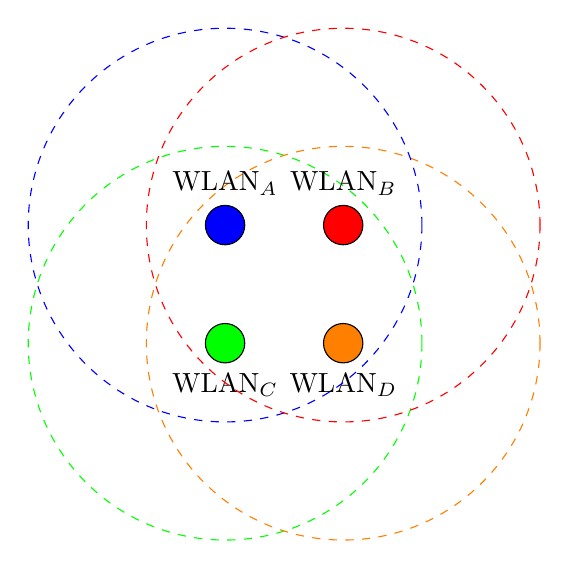
\begin{tikzpicture}
\node at (0,0) [circle, fill=green, draw, minimum width=0.5cm,minimum height=0.5cm, label=below:$\text{WLAN}_C$] (S1) {};
\node at (S1) [circle,draw=green, minimum size=5cm, dashed] (S1c) {};
\node[circle, fill=orange, draw, minimum width=0.5cm,minimum height=0.5cm, label=below:$\text{WLAN}_D$] (S2) [right of=S1, xshift=0.5cm] {};
\node at (S2) [circle,draw=orange, minimum size=5cm, dashed] (S2c) {};
\node[circle,draw, fill=blue, minimum width=0.5cm,minimum height=0.5cm, label=above:$\text{WLAN}_A$] (S3) [above of=S1, yshift=0.5cm] {};
\node at (S3) [circle,draw=blue, minimum size=5cm, dashed] (S3c) {};
\node[circle,draw, fill=red, minimum width=0.5cm,minimum height=0.5cm, label=above:$\text{WLAN}_B$] (S4) [above of=S2, yshift=0.5cm] {};
\node at (S4) [circle,draw=red, minimum size=5cm, dashed] (S4c) {};

\end{tikzpicture}
\caption{Coverage range for CTMN model with 4 WLANs.} \label{fig:ctmn_wlans_coverage}
\end{figure}

\begin{figure}[h]
\centering
  \begin{subfigure}[b]{0.475\textwidth}
    \centering
    \includegraphics[width=\textwidth]{img/channel_bonding_scenario1.png}
    \caption[]%
    {{\small Scenario 1}}    
    \label{fig:channel_bonding_scenario1}
  \end{subfigure}
  \hfill
  \begin{subfigure}[b]{0.475\textwidth}  
    \centering 
    \includegraphics[width=\textwidth]{img/channel_bonding_scenario2.png}
    \caption[]%
    {{\small Scenario 2}}
    \label{fig:channel_bonding_scenario2}
  \end{subfigure}
    \begin{subfigure}[b]{0.475\textwidth}
    \centering
    \includegraphics[width=\textwidth]{img/channel_bonding_scenario3.png}
    \caption[]%
    {{\small Scenario 3}}    
    \label{fig:channel_bonding_scenario3}
  \end{subfigure}
  \hfill
  \begin{subfigure}[b]{0.475\textwidth}  
    \centering 
    \includegraphics[width=\textwidth]{img/channel_bonding_scenario4.png}
    \caption[]%
    {{\small Scenario 4}}    
    \label{fig:channel_bonding_scenario4}
  \end{subfigure}
  \vskip\baselineskip
  \begin{subfigure}[b]{0.475\textwidth}   		
    \centering 
    \includegraphics[width=\textwidth]{img/channel_bonding_scenario5.png}
    \caption[]%
    {{\small Scenario 5}}    
    \label{fig:channel_bonding_scenario5}
  \end{subfigure}
  \quad
  \begin{subfigure}[b]{0.475\textwidth}   
    \centering 
    \includegraphics[width=\textwidth]{img/channel_bonding_scenario6.png}
    \caption[]%
    {{\small Scenario 6}}    
    \label{fig:channel_bonding_scenario6}
  \end{subfigure}
  \begin{subfigure}[b]{0.475\textwidth}   		
    \centering 
    \includegraphics[width=\textwidth]{img/channel_bonding_scenario7.png}
    \caption[]%
    {{\small Scenario 7}}    
    \label{fig:channel_bonding_scenario7}
  \end{subfigure}
  \quad
  \begin{subfigure}[b]{0.475\textwidth}   
    \centering 
    \includegraphics[width=\textwidth]{img/channel_bonding_scenario8.png}
    \caption[]%
    {{\small Scenario 8}}    
    \label{fig:channel_bonding_scenario8}
  \end{subfigure}
\caption[Channel allocations]
{\small Channel allocations of the different scenarios.} 
\label{fig:channel_allocation_3to6}
\end{figure}

\begin{table}[]
\centering
\caption{Summary of the results obtained for the \textit{log2} DCB scenarios. Throughput computations in Komondor slightly differ from CTMN ones at Scenario 4 (in red). This is because the CTMC model allows STA B to pick the range 2 - 3 while it is not permitted in the \textit{log2} model implemented in Komondor.}
\label{table:scenario_4wlans}
\begin{tabular}{|c|c|c|c|c|c|c|c|}
\hline
\textbf{Scenario}                           & \textbf{States}                              & \textbf{Tool} & $\Gamma_A$ & $\Gamma_B$ & $\Gamma_C$ & $\Gamma_D$ & $\Gamma$   \\ \hline
                                            &                                              & Komondor       & 57.6104    & 57.6225    & -          & -          & 115.2329   \\ \cline{3-8} 
\multirow{-2}{*}{1}                         & \multirow{-2}{*}{3}                          & CTMN          & 57.6166    & 57.6166    & -          & -          & 115.2331   \\ \hline
                                            &                                              & Komondor       & 62.6054    & 61.9511    & -          & -          & 124.5566   \\ \cline{3-8} 
\multirow{-2}{*}{2}                         & \multirow{-2}{*}{5}                          & CTMN          & 62.6145    & 61.9399    & -          & -          & 124.5544   \\ \hline
                                            &                                              & Komondor       & 31.3030    & 31.2908    & 62.1658    & -          & 124.7597   \\ \cline{3-8} 
\multirow{-2}{*}{3}                         & \multirow{-2}{*}{7}                          & CTMN          & 31.2965    & 31.2965    & 62.1671    & -          & 124.7601   \\ \hline
\rowcolor[HTML]{FFCCC9} 
\cellcolor[HTML]{FFCCC9}                    & \cellcolor[HTML]{FFCCC9}                     & Komondor       & 61.9338    & 62.914772  & 114.6460   & -          & 239.494597 \\ \cline{3-8} 
\rowcolor[HTML]{FFCCC9} 
\multirow{-2}{*}{\cellcolor[HTML]{FFCCC9}4} & \multirow{-2}{*}{\cellcolor[HTML]{FFCCC9}13} & CTMN          & 61.9390    & 63.1841    & 113.4185   & -          & 238.5416   \\ \hline
                                            &                                              & Komondor       & 41.3179    & 41.2383    & 41.2891    & 41.2491    & 165.0945   \\ \cline{3-8} 
\multirow{-2}{*}{5}                         & \multirow{-2}{*}{5}                          & CTMN          & 41.2737    & 41.2737    & 41.2737    & 41.2737    & 165.0947   \\ \hline
                                            &                                              & Komondor       & 57.6193    & 57.6136    & 57.6184    & 57.6152    & 230.4667   \\ \cline{3-8} 
\multirow{-2}{*}{6}                         & \multirow{-2}{*}{9}                          & CTMN          & 57.6166    & 57.6166    & 57.6166    & 57.6166    & 230.4663   \\ \hline
                                            &                                              & Komondor       & 57.6193    & 57.6136    & 57.6184    & 57.6152    & 230.4667   \\ \cline{3-8} 
\multirow{-2}{*}{7}                         & \multirow{-2}{*}{9}                          & CTMN          & 57.6166    & 57.6166    & 57.6166    & 57.6166    & 230.4663   \\ \hline
                                            &                                              & Komondor       & 41.3179    & 41.2383    & 41.2891    & 41.2491    & 165.0945   \\ \cline{3-8} 
\multirow{-2}{*}{8}                         & \multirow{-2}{*}{5}                          & CTMN          & 41.2737    & 41.2737    & 41.2737    & 41.2737    & 165.0947   \\ \hline
\end{tabular}
\end{table}

\begin{table}[]
\centering
\caption{Summary of the results obtained for the \textit{log2} DCB scenarios with ACK and WLANs implemented. Simulation time is 10,000 seconds. All scenarios properly replicated :D}
\label{table:scenario_4wlans}
\begin{tabular}{|c|c|c|c|c|c|c|c|}
\hline
\textbf{Scenario}                           & \textbf{States}                              & \textbf{Tool} & $\Gamma_A$ & $\Gamma_B$ & $\Gamma_C$ & $\Gamma_D$ & $\Gamma$   \\ \hline
                                            &                                              & ACK       & 57.1418    & 57.2815    & -          & -          & 114.4234   \\ \cline{3-8} 
\multirow{-2}{*}{1}                         & \multirow{-2}{*}{3}                          & CTMN          & 57.6166    & 57.6166    & -          & -          & 115.2331   \\ \hline
                                            &                                              & ACK       & 62.5831    & 61.3054   & -          & -          & 123.8886   \\ \cline{3-8} 
\multirow{-2}{*}{2}                         & \multirow{-2}{*}{5}                          & CTMN          & 62.6145    & 61.9399    & -          & -          & 124.5544   \\ \hline
                                            &                                              & ACK       & 31.1883    & 31.1394    & 61.7620    & -          & 124.0898   \\ \cline{3-8} 
\multirow{-2}{*}{3}                         & \multirow{-2}{*}{7}                          & CTMN          & 31.2965    & 31.2965    & 62.1671    & -          & 124.7601   \\ \hline
\rowcolor[HTML]{FFCCC9} 
\cellcolor[HTML]{FFCCC9}                    & \cellcolor[HTML]{FFCCC9}                     & ACK       & XXX    & XXX  & XXX   & -          & XXX \\ \cline{3-8} 
\rowcolor[HTML]{FFCCC9} 
\multirow{-2}{*}{\cellcolor[HTML]{FFCCC9}4} & \multirow{-2}{*}{\cellcolor[HTML]{FFCCC9}13} & CTMN          & 61.9390    & 63.1841    & 113.4185   & -          & 238.5416   \\ \hline
                                            &                                              & ACK       & 40.8806   & 40.8506    & 40.7439    & 40.7498    & 163.2251   \\ \cline{3-8} 
\multirow{-2}{*}{5}                         & \multirow{-2}{*}{5}                          & CTMN          & 41.2737    & 41.2737    & 41.2737    & 41.2737    & 165.0947   \\ \hline
                                            &                                              & ACK       & XXX    &XXX    & XXX    & XXX    & XXX   \\ \cline{3-8} 
\multirow{-2}{*}{6}                         & \multirow{-2}{*}{9}                          & CTMN          & 57.6166    & 57.6166    & 57.6166    & 57.6166    & 230.4663   \\ \hline
                                            &                                              & ACK       & XXX    & XXX    & XXX    & XXX    & XXX   \\ \cline{3-8} 
\multirow{-2}{*}{7}                         & \multirow{-2}{*}{9}                          & CTMN          & 57.6166    & 57.6166    & 57.6166    & 57.6166    & 230.4663   \\ \hline
                                            &                                              & ACK       & XXX   & XXX    &XXX1    & XXX   &XXX   \\ \cline{3-8} 
\multirow{-2}{*}{8}                         & \multirow{-2}{*}{5}                          & CTMN          & 41.2737    & 41.2737    & 41.2737    & 41.2737    & 165.0947   \\ \hline
\end{tabular}
\end{table}

The validation test seems satisfactory as the throughput computed with Komondor and the CTMN model are pretty similar.

%%%%%%%%%%%%%%%
% TUTORIAL
%%%%%%%%%%%%%%%
\section{Brief tutorial}
\begin{enumerate}
	\item Set the .csv input files (format explained in XXX)
	\item "cd" to \textit{KomondorSimulator} directory
    \item Execute ".build\_local". This file contains the instructions for compiling the Komondor code. It is also updated to enable debugging with Valgrind\footnote{Valgrind is a programming tool for memory debugging, memory leak detection, and profiling. Valgrind main website: \url{http://valgrind.org/}}.
    \item Execute \textit{./KomondorSimulator arg\_1 arg\_2 ... arg\_n}, where \textit{arg\_i} is the ith input argument.
    	\begin{itemize}
    		\item \textit{arg\_1}: simulation time [s]
    		\item \textit{arg\_2}: random seed [n.u]
            \item \textit{arg\_3}: activate node logs [boolean]\footnote{Major increases in the execution time may occur if nodes logging is activated. E.g., for a simulation of 4 nodes, simulating 1000 seconds takes 1.127 s and 15.672 s when not logging and when doing so, respectively.}
		\end{itemize}
    \item Write a paper with the results
    \item Be accepted :D
\end{enumerate}


\subsection{Console input}
Simulation time, seed...
\subsection{Input files}
Csv files that...
\begin{itemize}
  \item Nodes config: It is \textbf{mandatory} to enter and input file with a list of nodes ordered by \textit{node\_id} and starting with \textit{node\_id} = 0. It is needed for the array responsible of storing the power perceived by each node (i.e., \textit{power\_received\_per\_node}).
  \item System config
\end{itemize}
\subsection{Output files}
\begin{itemize}
	\item Node events logs: events are categorized as summarized in Table \ref{table:event_coding}. \textcolor{red}{More \textit{specific} (i.e., just numbers or identifiers - no description text) logs to be done.}
	\item Statistics
\end{itemize}

\begin{table}[]
\centering
\scriptsize
\caption{Node's event logs encoding.}
\label{table:event_coding}
\begin{tabular}{|c|c|c|c|}
\hline
\textbf{Method}                            & \textbf{Type}       & \textbf{Sub-type} & \textbf{Event description}                              \\ \hline
Setup()                                    & A                   & -                 & -                                                       \\ \hline
\multirow{3}{*}{Start()}                   & \multirow{3}{*}{B}  & B00               & Start()                                                 \\ \cline{3-4} 
                                           &                     & B01               & Start() end                                             \\ \cline{3-4} 
                                           &                     & B02               & Node's info (one line)                                  \\ \hline
\multirow{6}{*}{Stop()}                    & \multirow{6}{*}{C}  & C00               & Stop()                                                  \\ \cline{3-4} 
                                           &                     & C01               & Stop() end                                              \\ \cline{3-4} 
                                           &                     & C02               & Time transmitting in number of channels                 \\ \cline{3-4} 
                                           &                     & C03               & Time transmitting in each channel                       \\ \cline{3-4} 
                                           &                     & C04               & Packets sent                                            \\ \cline{3-4} 
                                           &                     & C05               & Throughput                                              \\ \hline
\multirow{14}{*}{inportSomeNodeStartTX()}  & \multirow{14}{*}{D} & D00               & inportSomeNodeStartTX()                                 \\ \cline{3-4} 
                                           &                     & D01               & inportSomeNodeStartTX() end                             \\ \cline{3-4} 
                                           &                     & D02               & Node N has started a TX in channels: c\_left - c\_right \\ \cline{3-4} 
                                           &                     & D03               & Pre update channel state                                \\ \cline{3-4} 
                                           &                     & D04               & Distance to transmitting node                           \\ \cline{3-4} 
                                           &                     & D05               & Power received from transmitting node                   \\ \cline{3-4} 
                                           &                     & D06               & Post update channel state                               \\ \cline{3-4} 
                                           &                     & D07               & I am (or not) the TX destination                        \\ \cline{3-4} 
                                           &                     & D08               & Current SINR                                            \\ \cline{3-4} 
                                           &                     & D09               & Capacitiy                                               \\ \cline{3-4} 
                                           &                     & D10               & Primary channel affected (or not)                       \\ \cline{3-4} 
                                           &                     & D11               & Power sensed in primary channel                         \\ \cline{3-4} 
                                           &                     & D12               & CCA exceeded (or not)                                   \\ \cline{3-4} 
                                           &                     & D13               & Backoof active (or not)                                 \\ \hline
\multirow{10}{*}{inportSomeNodeFinishTX()} & \multirow{10}{*}{E} & E00               & inportSomeNodeFinishTX()                                \\ \cline{3-4} 
                                           &                     & E01               & inportSomeNodeFinishTX() end                            \\ \cline{3-4} 
                                           &                     & E02               & N\%d has finished a TX in channel range: \%d - \%d      \\ \cline{3-4} 
                                           &                     & E03               & Initial power of transmitter                            \\ \cline{3-4} 
                                           &                     & E04               & Pre update channel state                                \\ \cline{3-4} 
                                           &                     & E05               & Post update channel state                               \\ \cline{3-4} 
                                           &                     & E06               & Primary channel affected (or not)                       \\ \cline{3-4} 
                                           &                     & E07               & Power sensed in primary channel                         \\ \cline{3-4} 
                                           &                     & E08               & CCA exceeded (or not)                                   \\ \cline{3-4} 
                                           &                     & E09               & I am transmitting (or not)                              \\ \hline
\multirow{6}{*}{endBackoff()}              & \multirow{6}{*}{F}  & F00               & endBackoff()                                            \\ \cline{3-4} 
                                           &                     & F01               & endBackoff() end                                        \\ \cline{3-4} 
                                           &                     & F02               & Channels for transmitting                               \\ \cline{3-4} 
                                           &                     & F03               & Transmission is possible (or not)                       \\ \cline{3-4} 
                                           &                     & F04               & Selected transmission range                             \\ \cline{3-4} 
                                           &                     & F05               & New backoff generated                                   \\ \hline
\multirow{3}{*}{myTXFinished()}            & \multirow{3}{*}{G}  & G00               & myTXFinished()                                          \\ \cline{3-4} 
                                           &                     & G01               & myTXFinished() end                                      \\ \cline{3-4} 
                                           &                     & G02               & New backoff generated                                   \\ \hline
\end{tabular}
\end{table}











\section{Code development}

This section is for code and structure clarifications that developers may need to remember or modify sometime. 

\subsection{Main considerations}
\begin{itemize}
\item \textbf{Power and CCA}: power variables are stored in pW (pico watts) in order to be able to operate power magnitudes without loosing resolution\footnote{E.g., the sum of two signals of power values -85 dBm (3.162 pW) and -90 dBm (1 pW), respectively, is -83.803 dBm (4.162 pW).}. However, values are presented to the user in dBm.

W (-30)  - mW (0)  - uW (+30) - nW (+60) - pW (+90)\\
$P_{\text{pw}} = 10^{\frac{P_{\text{dBm}} + 90}{10}}$
\end{itemize}

\subsection{Miscellany}
\begin{itemize}
\item Transmitting capability: we have added a flag to each node that determines if it is able to transmit (1) or not (0), so that we can decide if the node is only listening or both transmitting and listening.
\item Progress bar: the Komondor simulation progress bar is displayed through a \textit{printf()} command called by any node with \textit{node\_id} set to 0. If no node has \textit{node\_id} set to 0, the progress bar is not displayed.
\end{itemize}

\section{Releases}

\subsection{Komondor v0.1}
Features:
\begin{itemize}
\item Channel Bonding
\item Adjacent power
\item Collisions
\item Scripting
\item Path loss models
\end{itemize}

%-------------------------------
%-------------------------------
%-------------------------------
%-------------------------------

\section{Conclusions}
Does not apply yet.


\begin{thebibliography}{1}

\bibitem{ref:cost} 
Chen, Gilbert, and Boleslaw K. Szymanski. "Reusing simulation components: cost: a component-oriented discrete event simulator."
Proceedings of the 34th conference on Winter simulation: exploring new frontiers. Winter Simulation Conference, 2002.

\end{thebibliography}

\end{document}